\documentclass{amsart}
\renewcommand{\baselinestretch}{1.1}
\setlength{\parskip}{2mm}

\usepackage{amsthm}
\usepackage{amsmath}
\usepackage{amsfonts}
\usepackage{amssymb}
\usepackage{fullpage}
\usepackage{xcolor}
\usepackage{textcomp}
\usepackage{graphicx}

\newtheorem*{theirtheorem}{Theorem}
\newtheorem*{theirproposition}{Proposition}


\theoremstyle{plain}
\newtheorem*{theorem}{\textbf{Theorem}}
\newtheorem*{lemma}{\textbf{Lemma}}
\newtheorem*{corollary}{\textbf{Corollary}}
\newtheorem*{proposition}{\textbf{Proposition}}
\newtheorem*{claim}{\textbf{Claim}}
\newtheorem*{conjecture}{\textbf{Conjecture}}

\theoremstyle{definition}
\newtheorem*{rk}{\textbf{Remark}}

\newcommand{\Summ}[1]{\underset{#1}{\sum}}
\newcommand{\sti}[2]{\left\{\begin{array}{c} #1 \\ #2 \end{array}\right\}}

\newcommand{\diam}{\emph{diam}}
\newcommand{\conv}{\mbox{Conv}}
\newcommand{\C}{\mathcal {C}}
\newcommand{\R}{\mathbb{R}}
\newcommand{\Z}{\mathbb{Z}}
\newcommand{\N}{\mathbb{N}}
\newcommand{\F}{\mathbb{F}}

\newcommand{\B}{\mathcal{B}}
\newcommand{\A}{\mathcal{A}}
\newcommand{\G}{\mathcal{G}}
\newcommand{\D}{\mathcal{D}}

\newcommand{\ov}[1]{\overline{#1}}

\newcommand{\nn}{\nonumber}

\def\st{2}

\thispagestyle{empty}

\begin{document}

    {\Large Graph Theory -- MAMME}
    {\Large Chapter 1 -- Basics I}

    \vspace{0.5cm}

    \hrule

    \vspace{0.5cm}

    \noindent \textbf{Problem 6:}
    Let $G_1$ and $G_2$ be two Hamiltonian graphs.
    Show that $G_1 \square G_2$ is Hamiltonian.
    Show that the hypercube $Q^n$, for $n \geq 2$, is Hamiltonian.


    \paragraph{\textbf{Solution (by Ferran Espuña):}}
    Let $r = \lvert E(G_1)\rvert$, $s = \lvert E(G_2)\rvert$ and let
    \begin{alignat*}{0}
    & x_1, \, & x_2, \, & \ldots, \, & x_{r-1}, \, & x_r, \, & x_1 \\
    & y_1, \, & y_2, \, & \ldots, \, & y_{s-1}, \, & y_s, \, & y_1
    \end{alignat*}
    be Hamiltonian cycles in $G_1$ and $G_2$, respectively.
    We will construct a Hamiltonian cycle in $G_1 \square G_2$ as follows:

    \begin{itemize}
        \item We will course a path moving back and forth between $y_1$ and $y_{s-1}$ in each copy of $G_2$,
    hopping to the next copy using an edge of the form $(x_i, y_1) \sim (x_{i+1}, y_{1})$ or
    $(x_i, y_{s-1}) \sim (x_{i+1}, y_{s-1})$,
    and always leaving out $y_s$ in each copy so that we can use them later to go back to the original copy (indexed by $x_1$).
        \item Then, we will move to $(x_r, y_s)$ and, as said, go back to the original copy of $G_2$ using only copies of $y_s$ and reaching $(x_1, y_s)$
        \item Finally, we can go back to the original copy of $x_1$, thus completing the cycle.
    \end{itemize}

    \begin{proposition}\label{prop:1}
        The cartesian product of two Hamiltonian graphs is Hamiltonian.
        \begin{proof}
            \vspace{-6mm}
            Let's assume the notation for the cycles in $G_1$ and $G_2$ as above.
            The specifics vary depending on whether $r$ is even or odd, so we will show the full path if it is odd:
             \begin{alignat*}{0}
                    & \color{red} (x_1, y_1),\, && \color{red} (x_1, y_2),\, && \color{red} \ldots , \, (x_1, y_{s-1}),  \\
                    & (x_2, y_{s-1}),\, && (x_2, y_{s-2}),\, && \ldots , \,  (x_2, y_1), \\
                    & \color{red} (x_3, y_1),\, && \color{red} (x_3, y_2),\, && \color{red} \ldots, \,(x_3, y_{s-1}),  \\
                    & (x_4, y_{s-1}),\, && (x_4, y_{s-2}),\, && \ldots , \,  (x_4, y_1),  \\
                    &&&&& \ldots  \\
                    & \color{red}(x_r, y_1),\, && \color{red}(x_r, y_2),\, && \color{red}\ldots, \,  (x_r, y_{s-1}), \\
                    & \color{blue} (x_r, y_s), \\
                    & \color{blue} (x_{r-1}, y_s),\, && \color{blue} (x_{r-2}, y_{s}),\, && \color{blue} \ldots, \color{blue} \,  (x_1, y_s), \\
                    & \color{darkgray}(x_1, y_1) &&&&
             \end{alignat*}
            All vertices of the form $(x_i, y_j)$ where
            $j \neq s$ are covered exactly once in the black or \color{red} red \color{black} rows
            (except for $(x_1, y_1)$, which is both at the beginning and the end)
            and the rest are in the \color{blue} blue \color{black} \color{black} ones.
            All edges between adjacent nodes in the cycle are in the cartesian product by definition.
            If $r$ is even, we only need to change the last \color{red} red \color{black} row to a black one:
            \begin{alignat*}{0}
                 (x_r, y_{s-1}),\, & (x_r, y_{s-2}),\, & \ldots, \, &(x_r, y_1)
            \end{alignat*}
            But because both $y_1$ and $y_{s-1}$ are connected to $y_s$, this is fine.
                \end{proof}
    \end{proposition}

    \begin{figure}[!tbp]
        \centering
        \begin{minipage}[t]{0.49\textwidth}
            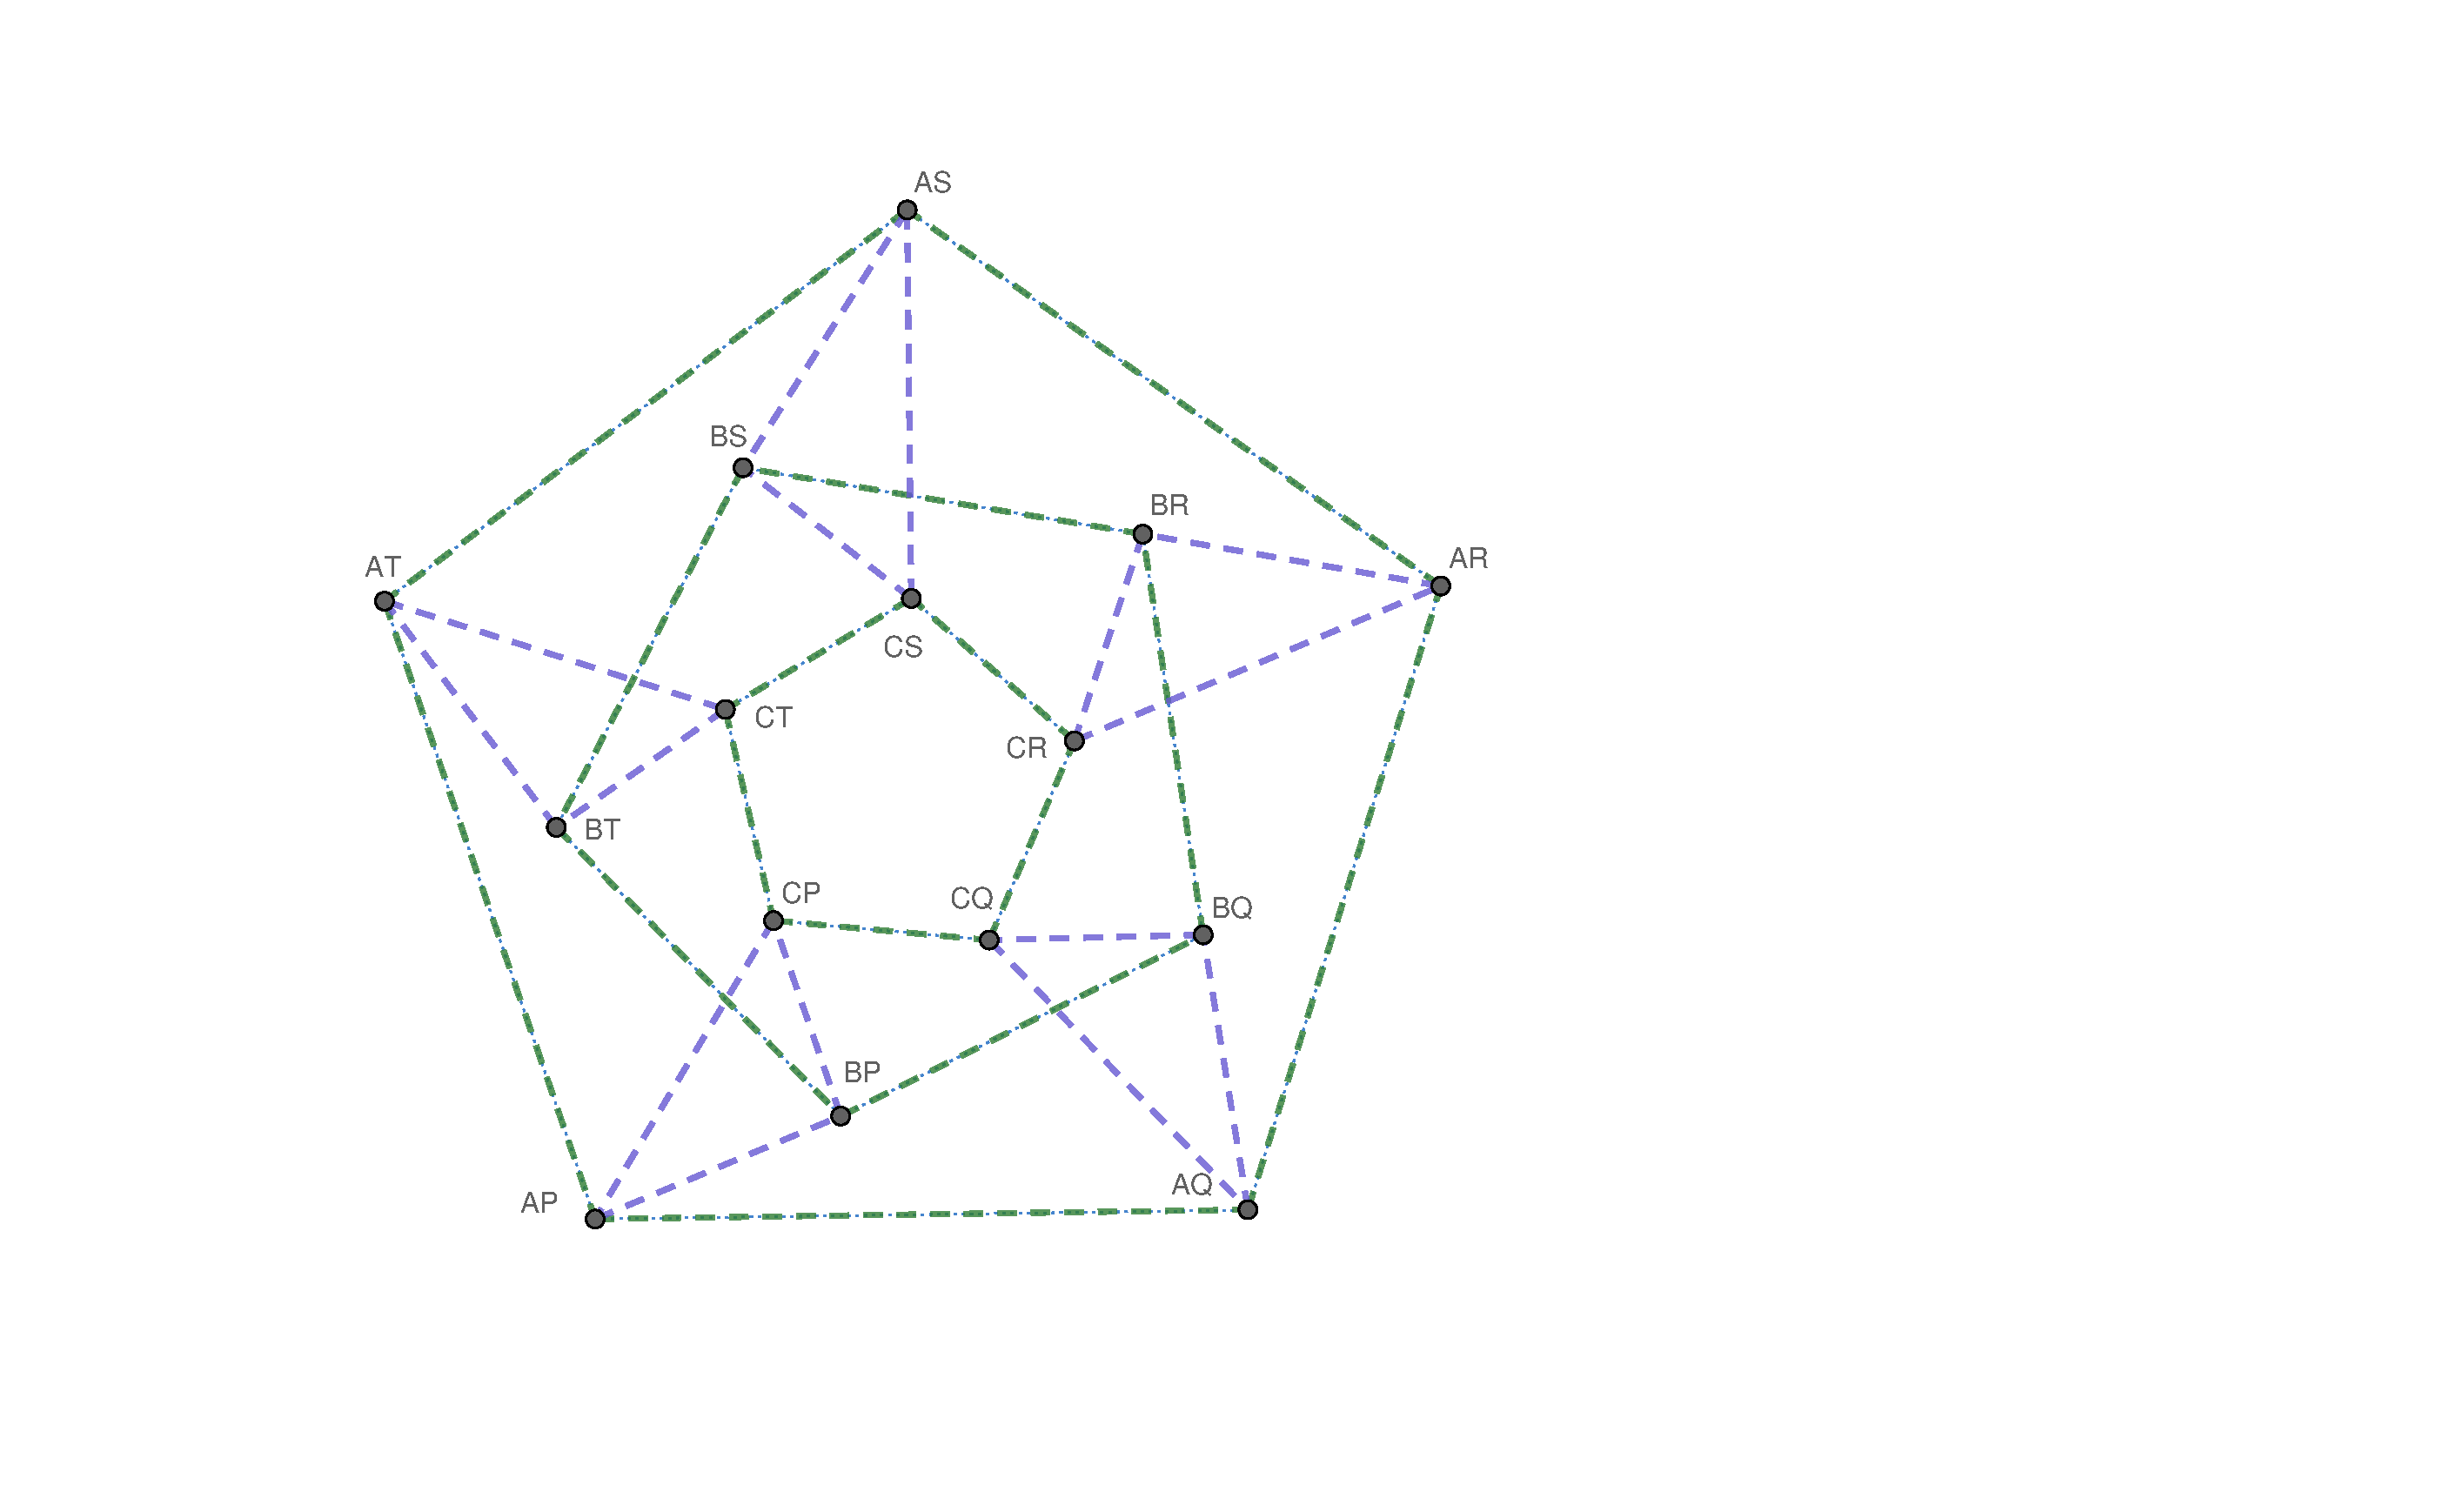
\includegraphics[width=\textwidth, trim={6.5cm 5cm 18.5cm 3cm},clip]{media/product}
            \caption{$G_1 \square G_2$ where $G_1$ is the $3$-cycle $ABC$ and $G_2$ is the $5$-cycle
            $PQRST$. \color[HTML]{6557D2} Violet \color{black} edges are the ones corresponding
            to copies of $G_1$ and \color[HTML]{2E7D32} green \color{black} edges are the ones corresponding to copies of $G_2$.}
        \end{minipage}
        \hfill
        \begin{minipage}[t]{0.49\textwidth}
            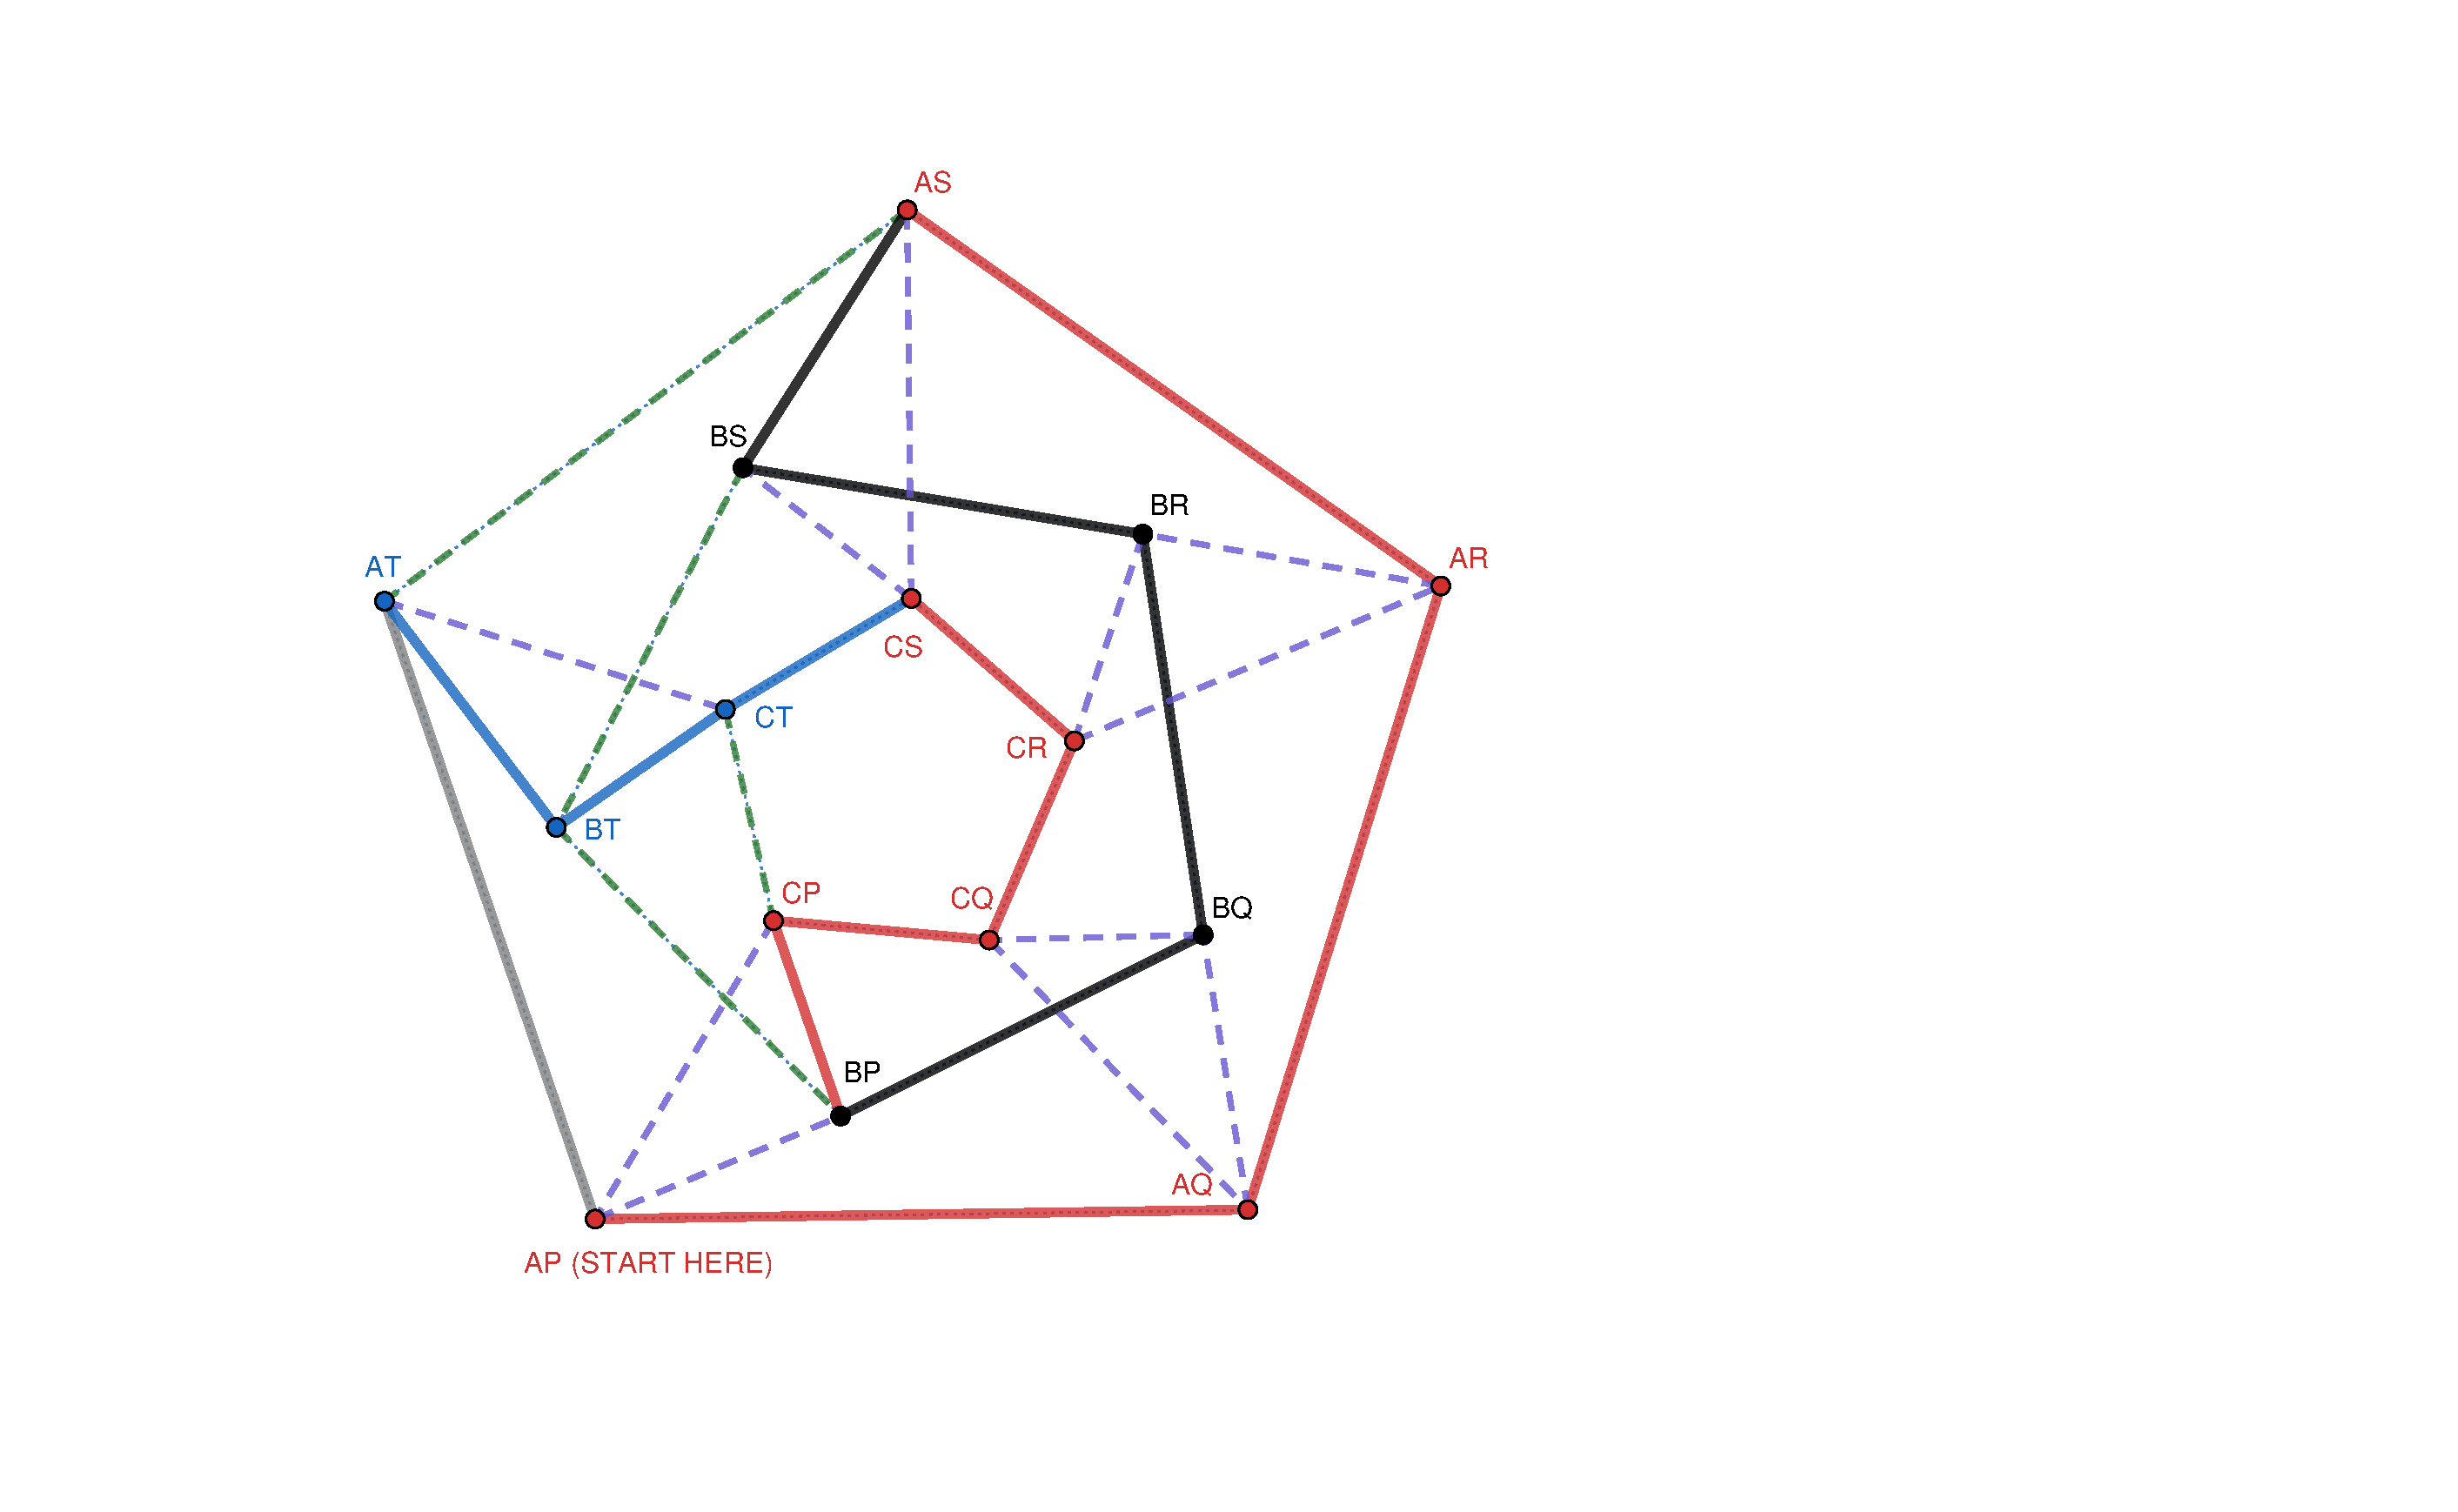
\includegraphics[width=\textwidth, trim={6.5cm 4.5cm 18.5cm 3cm},clip]{media/path}
            \caption{Hamiltonian path constructed in the proposition above, starting at $AP$. Edges are colored the same color as their endpoint in the proposition.}
        \end{minipage}

    \label{fig:figure}
    \end{figure}

    \begin{rk}
        The case for $r$ even can be made easier by just doing
        \begin{alignat*}{0}
            & (x_1, y_1),\, && (x_1, y_2),\, && \ldots, \, & (x_1, y_s), & \\
            & (x_2, y_s),\, && (x_2, y_{s-1}),\, && \ldots, \,  & (x_2, y_1), & \\
            & (x_3, y_1),\, && (x_3, y_2),\, && \ldots, \, & (x_3, y_s), & \\
            &&&&& \ldots \\
            & (x_r, y_s),\, && (x_r, y_{s-1}),\, && \ldots, \,  & (x_r, y_1), & \\
            & (x_1, y_1) &&&&&&
        \end{alignat*}
        But I did the other method because it works in both cases.
    \end{rk}
    \noindent Now, to tackle the hypercube $Q^n$, we just need to put it as the cartesian product of two hamiltonian graphs:
    \begin{proposition}
        The hypercube $Q^n$ is Hamiltonian.
        \begin{proof}
            Assume the notation $V(Q^1) = \{0, 1\}$, $V(Q^n) = \{0, 1\}^n$.
            We proceed by induction:
            \begin{itemize}
                \item For $n \in \{2, 3\}$, just construct the cycles ``by hand'':
                \begin{itemize}
                    \item $(0, 0), (0, 1), (1, 1), (1, 0), (0, 0)$
                    \item $(0, 0, 0), (0, 0, 1), (0, 1, 1), (0, 1, 0), (1, 1, 0), (1, 1, 1), (1, 0, 1), (1, 0, 0), (0, 0, 0)$
                \end{itemize}
                \item For higher $n$, we can use the fact that $Q^n \cong Q^{n-2} \square Q^2$, which is Hamiltonian by the previous proposition.
            \end{itemize}
        \end{proof}
    \end{proposition}

    \begin{rk}
        If we look at the structure of the two cycles we constructed for $Q^2$ and $Q^3$,
        we can find a somewhat simpler method for constructing the cycle for $Q^n$.
        In fact, we can show the following:
        \begin{claim}
            The cartesian product of any graph $G$ with a spanning path and $Q^1$ is Hamiltonian.
            \begin{proof}
                We denote $V(Q^1) = \{0, 1\}$ and let
                \begin{alignat*}{0}
                    y_1, y_2, \ldots, y_s
                \end{alignat*}
                be a spanning path in $G$.
                We can construct a Hamiltonian cycle in $Q^1 \square G$ as follows:
                \begin{alignat*}{0}
                    & (0, y_1),\, && (0, y_2),\, & \ldots,\, & (0, y_s), \\
                    & (1, y_s),\, && (1, y_{s-1}),\, & \ldots,\, & (1, y_1),\\
                    & (0, y_1) &&&&
                \end{alignat*}
            \end{proof}
        \end{claim}
    \noindent Because $Q^1$ clearly has a spanning path, we can use this claim to show that $Q^n$ is Hamiltonian for all $n \geq 2$ by induction (as we did before).
    \end{rk}


\end{document}

